\documentclass{article}
\usepackage{amsmath, amssymb, tikz}
\usepackage{xcolor, colortbl}
\usepackage{multicol}
\usepackage{longtable}


\renewcommand{\L}{\mathcal{L}}

\begin{document}
\begin{flushleft}
   \begin{center}
      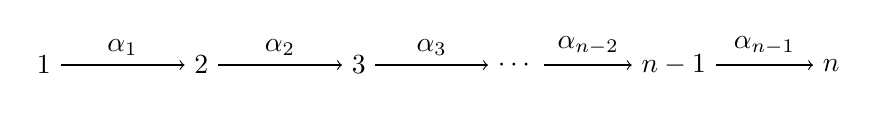
\begin{tikzpicture}
         \node (A) at (0,0) {1};
         \node (B) at (2,0) {2};
         \node (C) at (4,0) {3};
         \node (D) at (6,0) {$\cdots$};
         \node (E) at (8,0) {$n-1$};
         \node (F) at (10,0) {$n$};
         \draw[->] (A) -- (B) node[midway, anchor=south] {$\alpha_1$};
         \draw[->] (B) -- (C) node[midway, anchor=south] {$\alpha_2$};
         \draw[->] (C) -- (D) node[midway, anchor=south] {$\alpha_3$};
         \draw[->] (D) -- (E) node[midway, anchor=south] {$\alpha_{n-2}$};
         \draw[->] (E) -- (F) node[midway, anchor=south] {$\alpha_{n-1}$};
      \end{tikzpicture}
   \end{center}
   \begin{center}
      \begin{longtable}{|c|c|c|c|c|}
         \hline
         $n$ & Ideal & \texttt{V1} & \texttt{V2} & \texttt{V3} \\
         \hline 
         %%%%%%%%%%%%%%%%%%%%%%%%%%%%%%%%%%%%%%%%%%%%%%%%%%%%%%%%%
         %%%%%%%%%%%%%%%%%%%%%%%%%%%%%%%%%%%%%%%%%%%%%%%%%%%%%%%%%
         %%%%%%%%%%%%%%%%%%%%%%%%%%%%%%%%%%%%%%%%%%%%%%%%%%%%%%%%%
         3 & $(a_1a_2)$ & 6 & & 6\\
         \hline
         %%%%%%%%%%%%%%%%%%%%%%%%%%%%%%%%%%%%%%%%%%%%%%%%%%%%%%%%%
         %%%%%%%%%%%%%%%%%%%%%%%%%%%%%%%%%%%%%%%%%%%%%%%%%%%%%%%%%
         %%%%%%%%%%%%%%%%%%%%%%%%%%%%%%%%%%%%%%%%%%%%%%%%%%%%%%%%%
         4 & $(a_1a_2)$ & 8 & & 8\\
         & $(a_2a_3)$ & 8 && 8\\
         & $(a_1a_2, a_2a_3)$ & 8 && 8\\
         \rowcolor{blue!30!white}
         & $(a_1a_2a_3)$ & 10 && 5\\
         %%%%%%%%%%%%%%%%%%%%%%%%%%%%%%%%%%%%%%%%%%%%%%%%%%%%%%%%%
         %%%%%%%%%%%%%%%%%%%%%%%%%%%%%%%%%%%%%%%%%%%%%%%%%%%%%%%%%
         %%%%%%%%%%%%%%%%%%%%%%%%%%%%%%%%%%%%%%%%%%%%%%%%%%%%%%%%%
         5 & $(a_1a_2)$ & 10 && 10\\
         & $(a_2a_3)$ & 10 && 10 \\
         & $(a_3a_4)$ & 10 && 10\\
         & $(a_1a_2, a_2a_3)$ & 10 && 10 \\
         & $(a_1a_2, a_3a_4)$ & 10 && 10 \\
         & $(a_1a_2, a_2a_3, a_3a_4)$ & 10 && 10 \\
         & $(a_1a_2a_3)$ & 14 && 14\\
         & $(a_2a_3a_4)$ & 14 && 14\\
         & $(a_1a_2a_3, a_2a_3a_4)$ & 14 && 14\\
         & $(a_1a_2a_3a_4)$ & 14 && 14\\
         \hline
         %%%%%%%%%%%%%%%%%%%%%%%%%%%%%%%%%%%%%%%%%%%%%%%%%%%%%%%%%
         %%%%%%%%%%%%%%%%%%%%%%%%%%%%%%%%%%%%%%%%%%%%%%%%%%%%%%%%%
         %%%%%%%%%%%%%%%%%%%%%%%%%%%%%%%%%%%%%%%%%%%%%%%%%%%%%%%%%
         6 & $(a_1a_2)$ & 12 && 12 \\
         & $(a_2a_3)$ & 12 && 12 \\
         & $(a_3a_4)$ & 12 && 12 \\
         & $(a_4a_5)$ & 12 && 12 \\
         & $(a_1a_2, a_2a_3)$ & 12 && 12 \\
         & $(a_1a_2, a_3a_4)$ & 12 && 12 \\
         & $(a_1a_2, a_4a_5)$ & 12 && 12 \\
         & $(a_2a_3, a_3a_4)$ & 12 && 12 \\
         & $(a_2a_3, a_4a_5)$ & 12 && 12 \\
         & $(a_3a_4, a_4a_5)$ & 12 && 12 \\
         & $(a_1a_2, a_2a_3, a_3a_4)$ & 12 && 12 \\
         & $(a_1a_2, a_2a_3, a_4a_5)$ & 12 && 12 \\
         & $(a_1a_2, a_3a_4, a_4a_5)$ & 12 && 12 \\
         & $(a_2a_3, a_3a_4, a_4a_5)$ & 12 && 12 \\
         & $(a_1a_2, a_2a_3, a_3a_4, a_4a_5)$ & 12 && 12 \\
         & $(a_1a_2a_3)$ && 9 & 9 \\
         \rowcolor{blue!30!white}
         & $(a_2a_3a_4)$ && 11 & 22\\
         & $(a_3a_4a_5)$ && 9 & 9\\
         & $(a_1a_2a_3, a_2a_3a_4)$ && 9 & 9 \\
         \rowcolor{red!30!white}
         & $(a_1a_2a_3, a_3a_4a_5)$ && $>30$ & $>50$ \\
         & $(a_2a_3a_4, a_3a_4a_5)$ && 9 & 9\\
         & $(a_1a_2a_3, a_2a_3a_4, a_3a_4a_5)$ && 22 & 22 \\
         & $(a_1a_2a_3a_4)$ && 22 & 22\\
         & $(a_2a_3a_4a_5)$ && 22 & 22\\
         & $(a_1a_2a_3a_4, a_2a_3a_4a_5)$ && 22 & 22\\
         & $(a_1a_2a_3a_4a_5)$ && 9 & 9\\
         \hline
         %%%%%%%%%%%%%%%%%%%%%%%%%%%%%%%%%%%%%%%%%%%%%%%%%%%%%%%%%
         %%%%%%%%%%%%%%%%%%%%%%%%%%%%%%%%%%%%%%%%%%%%%%%%%%%%%%%%%
         %%%%%%%%%%%%%%%%%%%%%%%%%%%%%%%%%%%%%%%%%%%%%%%%%%%%%%%%%
         7 & $\ell_2$ &&& 14 \\
         & $(a_1a_2a_3a_4)$ &&& 17 \\
         \rowcolor{red!30!white}
         & $(a_2a_3a_4a_5)$ &&& $>50$ \\
         & $(a_3a_4a_5a_6)$ &&& 17 \\
         & $(a_1a_2a_3a_4, a_2a_3a_4a_5)$ &&& 17 \\
         \rowcolor{red!30!white}
         & $(a_1a_2a_3a_4, a_3a_4a_5a_6)$ &&& $>50$ \\
         & $(a_2a_3a_4a_5, a_3a_4a_5a_6)$ &&& 17 \\
         & $(a_1a_2a_3a_4, a_2a_3a_4a_5, a_3a_4a_5a_6)$ &&& 17 \\
         & $\ell_5$ &&& 17 \\
         & $\ell_6$ &&& 17 \\
         \hline
         %%%%%%%%%%%%%%%%%%%%%%%%%%%%%%%%%%%%%%%%%%%%%%%%%%%%%%%%%
         %%%%%%%%%%%%%%%%%%%%%%%%%%%%%%%%%%%%%%%%%%%%%%%%%%%%%%%%%
         %%%%%%%%%%%%%%%%%%%%%%%%%%%%%%%%%%%%%%%%%%%%%%%%%%%%%%%%%
         8 & $\ell_2 \setminus \{\lambda\}$ && 16 & 16\\
         \rowcolor{blue!30!white}
         & $\lambda = (a_1a_2, a_2a_3, a_3a_4, a_4a_5, a_5a_6, a_6a_7)$ && 8 & 16 \\
         & $(a_1a_2a_3) &&& 13 \\
         & $(a_2a_3a_4) &&& 29 \\
         \rowcolor{red!30!white}
         & $(a_3a_4a_5) &&& $>50$ \\
         & $(a_4a_5a_6) &&&  ?\\
         & $(a_5a_6a_7) &&&  ?\\
         \hline
         9 & $\ell_2$ &&& 18 \\
           & $\ell_7$ &&& $>50$ \\
           & $\ell_8$ &&& 30 \\
      \end{longtable}
   \end{center}
   \textbf{Conjecture 1:} If the ideal $I$ fails for $n$, it fails for all $N > n$. \\
   \textbf{Conjecture 2:} Ideals corresponding to length two relations never fail for any $n$. \\
   \textbf{Conjecture 3:} The dimension of ideals corresponding to length two relations is always $2n$.
\end{flushleft}
\end{document}
